\documentclass{cshwk}

\title{Principles of Database Systems\\Assignment \#4 - Structured Query Language 3}

\begin{document}
\maketitle


\section{Execute the SQL in Slides}

\subsection{Preparation}

\subsubsection{Create Table}

\begin{lstlisting}[language=sql]
CREATE TABLE movieexec
(
    name     CHAR(30),
    address  VARCHAR(255),
    cert     INT,
    networth INT
);
CREATE TABLE moviestar
(
    name      CHAR(30),
    address   VARCHAR(255),
    gender    CHAR(1),
    birthdate date
);
CREATE TABLE starsin
(
    movietitle CHAR(100),
    movieyear  INT,
    starname   CHAR(30)
);
CREATE TABLE Movies
(
    title      CHAR(100),
    year       INT,
    length     INT,
    genre      CHAR(10),
    studioName CHAR(30),
    producerC  INT,
    PRIMARY KEY (title, year)
);
CREATE TABLE studio
(
    name    CHAR(50) PRIMARY KEY,
    address VARCHAR(255),
    presc   INT
);
\end{lstlisting}

the execution results are shown in Figure \ref{fig:create-table}.

\begin{figure}[H]
    \centering
    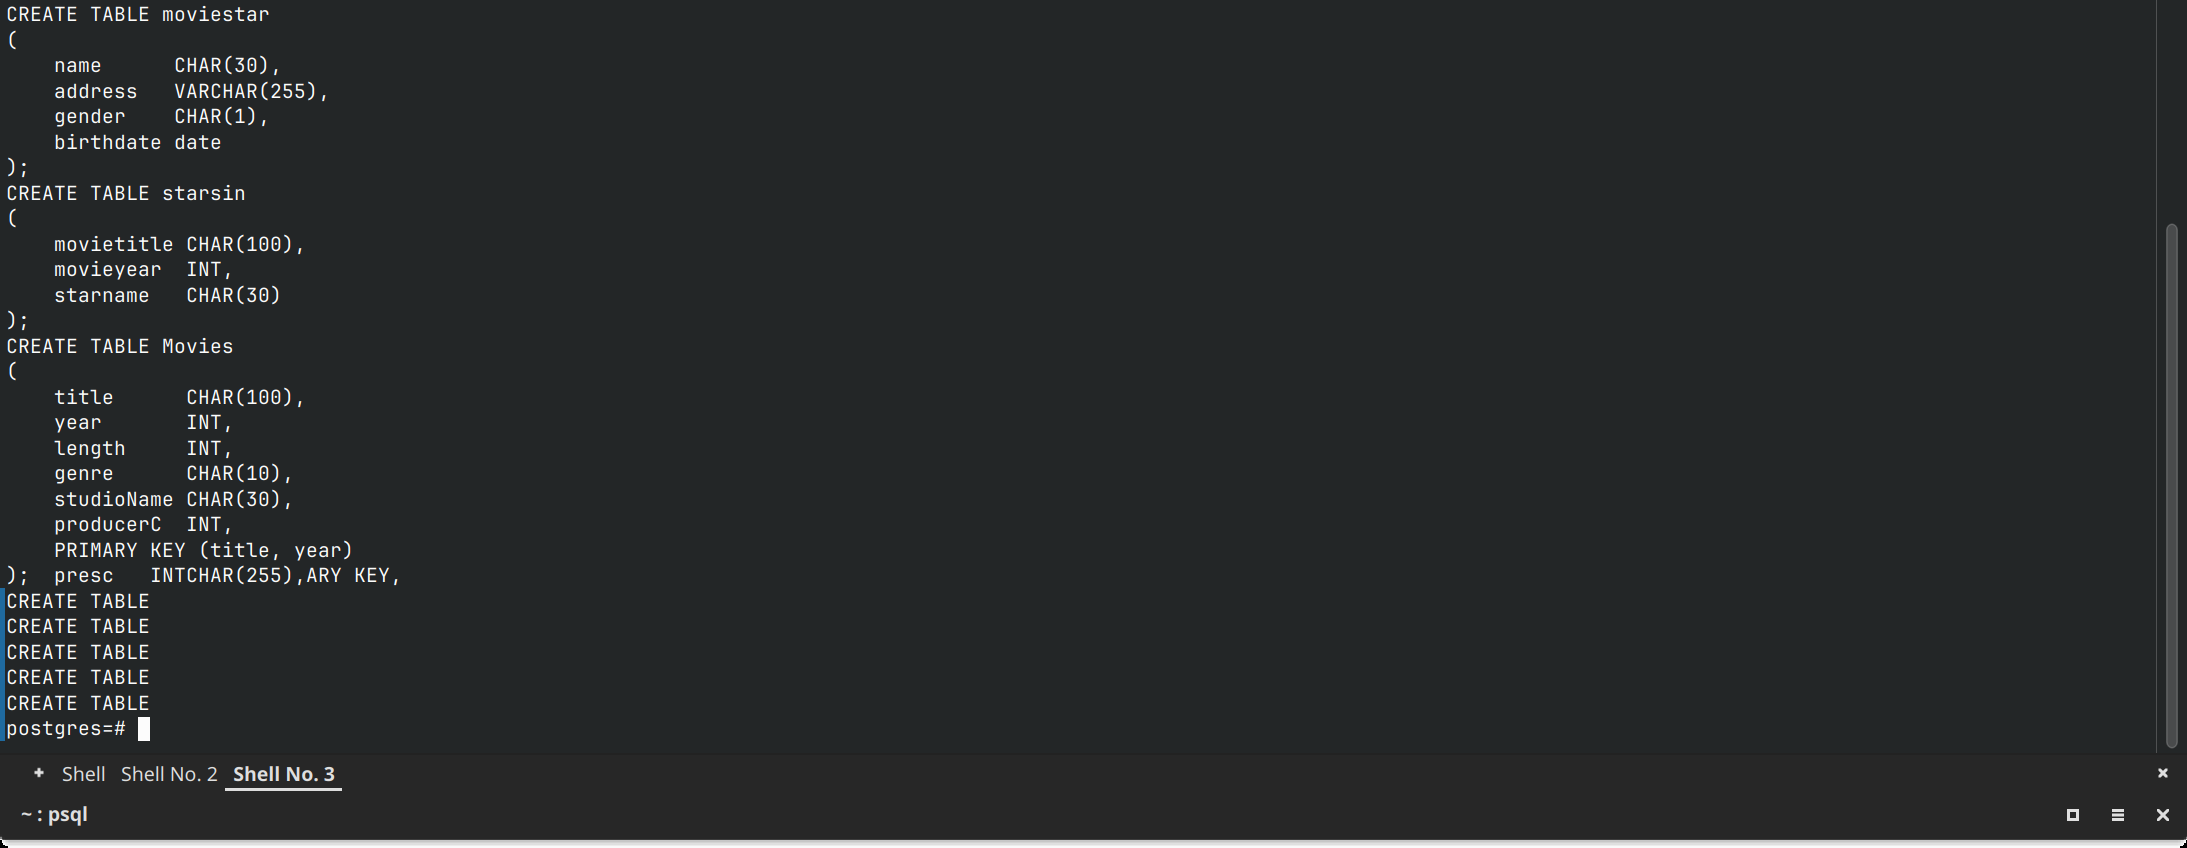
\includegraphics[width=0.8\textwidth]{hw6-1.png}
    \caption{Create Table}
    \label{fig:create-table}
\end{figure}

\subsubsection{Insert Data}

\begin{lstlisting}[language=sql]
INSERT INTO movies VALUES ('Logan''s run', 1976, NULL, 'sciFi', 'MGM', 123);
INSERT INTO movies VALUES ('Star Wars', 1977, 124, 'sciFi', 'Fox', 555);
INSERT INTO movies VALUES ('Empire Strikes Back', 1980, 111, 'fantasy', 'Fox', 555);
INSERT INTO movies VALUES ('Star Trek', 1979, 132, 'sciFi', 'Paramount', 345);
INSERT INTO movies VALUES ('Star Trek: Nemesis', 2002, 116, 'sciFi', 'Paramount', 345);
INSERT INTO movies VALUES ('Terms of Endearment', 1983, 132, 'romance', 'MGM', 123);
INSERT INTO movies VALUES ('The Usual Suspects', 1995, 106, 'crime', 'MGM', 456);
INSERT INTO movies VALUES ('Gone With the Wind', 1938, 238, 'drama', 'MGM', 123);
INSERT INTO movies VALUES ('Wayne''s World', 1992, 95, 'comedy', 'Paramount', 123);
INSERT INTO movies VALUES ('King Kong', 2005, 187, 'drama', 'Universal', 789);
INSERT INTO movies VALUES ('King Kong', 1976, 134, 'drama', 'Paramount', 666);
INSERT INTO movies VALUES ('King Kong', 1933, 100, 'drama', 'Universal', 345);
INSERT INTO movies VALUES ('Pretty Woman', 1990, 119, 'comedy', 'Disney', 999);

INSERT INTO movieexec VALUES ('George Lucas', 'Oak Rd.', 555, 200000000);
INSERT INTO movieexec VALUES ('Ted Turner', 'Turner Av.', 333, 125000000);
INSERT INTO movieexec VALUES ('Stephen Spielberg', '123 ET road', 222, 100000000);
INSERT INTO movieexec VALUES ('Merv Griffin', 'Riot Rd.', 199, 112000000);
INSERT INTO movieexec VALUES ('Calvin Coolidge', 'Fast Lane', 123, 20000000);
INSERT INTO movieexec VALUES ('Garry Marshall', 'First Street', 999, 50000000);
INSERT INTO movieexec VALUES ('J.J. Abrams', 'High Road', 345, 45000000);
INSERT INTO movieexec VALUES ('Bryan Singer', 'Downtown', 456, 70000000);
INSERT INTO movieexec VALUES ('George Roy Hill', 'Baldwin Av.', 789, 20000000);
INSERT INTO movieexec VALUES ('Dino De Laurentiis', ' Beverly Hills', 666, 120000000);
INSERT INTO movieexec VALUES ('AAA', ' Beverly Hills', 666, 120000000);

INSERT INTO moviestar VALUES ('Jane Fonda', 'Turner Av.', 'F', '1977-07-07');
INSERT INTO moviestar VALUES ('Alec Baldwin', 'Baldwin Av.', 'M', '1977-06-07');
INSERT INTO moviestar VALUES ('Kim Basinger', 'Baldwin Av.', 'F', '1979-05-07');
INSERT INTO moviestar VALUES ('Harrison Ford', 'Beverly Hills', 'M', '1977-07-07');
INSERT INTO moviestar VALUES ('Carrie Fisher', '123 Maple St.', 'F', '1999-09-09');
INSERT INTO moviestar VALUES ('Mark Hamill', '456 Oak Rd.', 'M', '1988-08-08');
INSERT INTO moviestar VALUES ('Debra Winger', 'A way', 'F', '1978-05-06');
INSERT INTO moviestar VALUES ('Jack Nicholson', 'X path', 'M', '1949-05-05');
INSERT INTO moviestar VALUES ('Kevin Spacey', 'New York Av.', 'F', '1937-12-21');
INSERT INTO moviestar VALUES ('AAA', 'New York Av.', 'F', '1937-12-21');

INSERT INTO starsin VALUES ('Star Wars', 1977, 'Carrie Fisher');
INSERT INTO starsin VALUES ('Star Wars', 1977, 'Mark Hamill');
INSERT INTO starsin VALUES ('Star Wars', 1977, 'Harrison Ford');
INSERT INTO starsin VALUES ('Empire Strikes Back', 1980, 'Harrison Ford');
INSERT INTO starsin VALUES ('The Usual Suspects', 1995, 'Kevin Spacey');
INSERT INTO starsin VALUES ('Terms of Endearment', 1983, 'Debra Winger');
INSERT INTO starsin VALUES ('Terms of Endearment', 1983, 'Jack Nicholson');

INSERT INTO studio VALUES ('MGM','MGM Boulevard', 123);
INSERT INTO studio VALUES ('Fox', 'Hollywood', 555);
INSERT INTO studio VALUES ('Disney', 'Buena Vista', 999);
INSERT INTO studio VALUES ('Paramount', 'Hollywood', 345);
INSERT INTO studio VALUES ('Universal', 'Hollywood', 789);
\end{lstlisting}

\subsection{Aggregation Operators}

\begin{lstlisting}[language=sql]
SELECT AVG(netWorth) FROM MovieExec;

SELECT SUM(netWorth) FROM MovieExec;

SELECT MIN(netWorth) FROM MovieExec;

SELECT MAX(netWorth) FROM MovieExec;

SELECT COUNT(*) FROM StarsIn;

SELECT COUNT(starName) FROM StarsIn;

SELECT COUNT(DISTINCT starName) FROM StarsIn;
\end{lstlisting}

The execution results are shown in Figure \ref{fig:aggregation-operators}.
\begin{figure}[H]
    \centering
    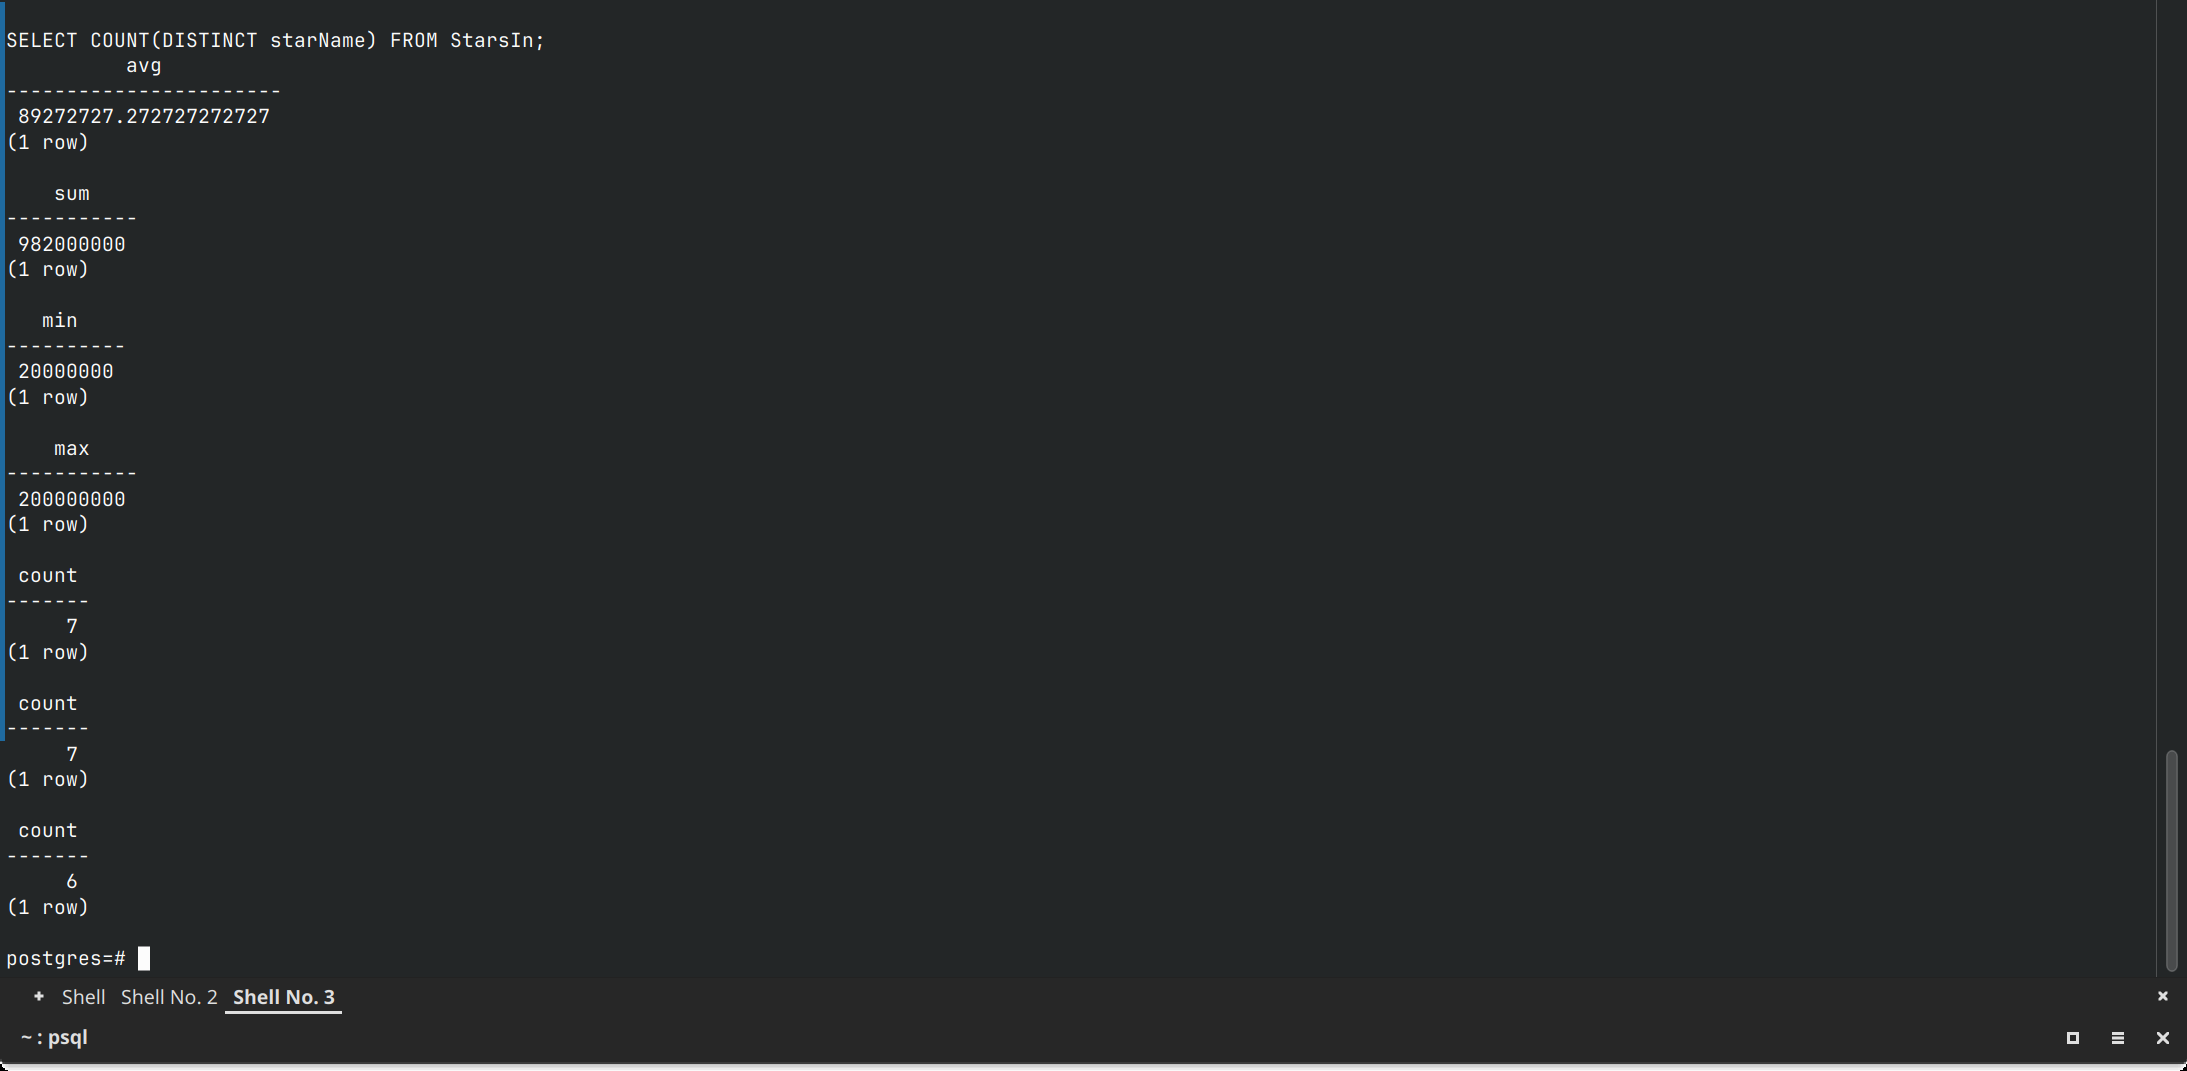
\includegraphics[width=0.8\textwidth]{hw6-2.png}
    \caption{Aggregation Operators}
    \label{fig:aggregation-operators}
\end{figure}

\subsection{Grouping}

\begin{lstlisting}[language=sql]
SELECT studioName, SUM(length) FROM Movies
GROUP BY studioName;

SELECT studioName, SUM(length), Count(length), AVG(length) FROM Movies
GROUP BY studioName;

SELECT studioName, Count(*) FROM Movies
GROUP BY studioName;

SELECT studioName FROM Movies
GROUP BY studioName;
\end{lstlisting}

The execution results are shown in Figure \ref{fig:grouping}.
\begin{figure}[H]
    \centering
    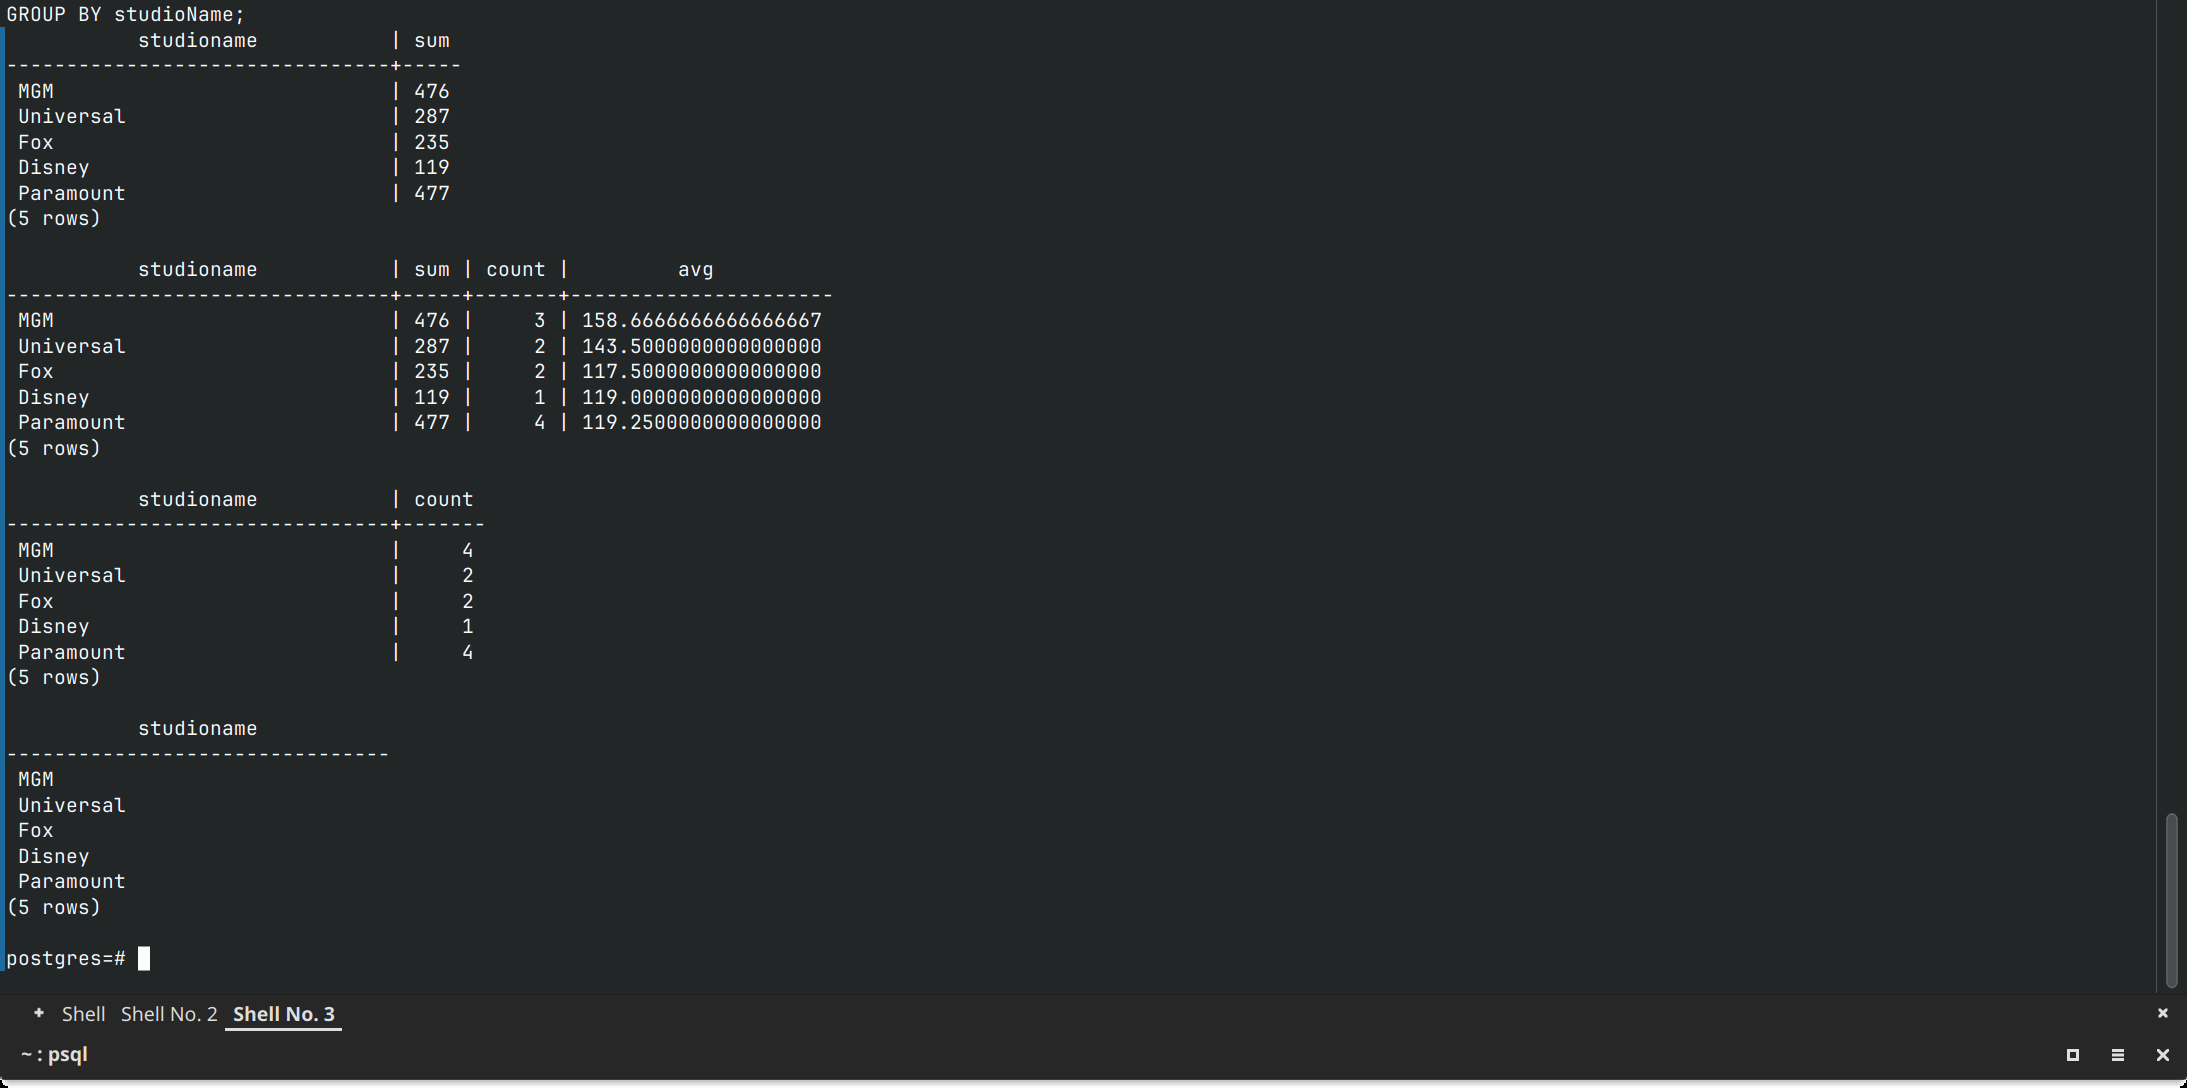
\includegraphics[width=0.8\textwidth]{hw6-3.png}
    \caption{Grouping}
    \label{fig:grouping}
\end{figure}

\subsection{Grouping with More Than One Relation}

\begin{lstlisting}[language=sql]
SELECT name, SUM(length)
FROM MovieExec,
     Movies
WHERE producerC = cert
GROUP BY name;

SELECT name, Count(*)
FROM MovieExec,
     Movies
WHERE producerC = cert
GROUP BY name;
\end{lstlisting}

\begin{figure}
    \centering
    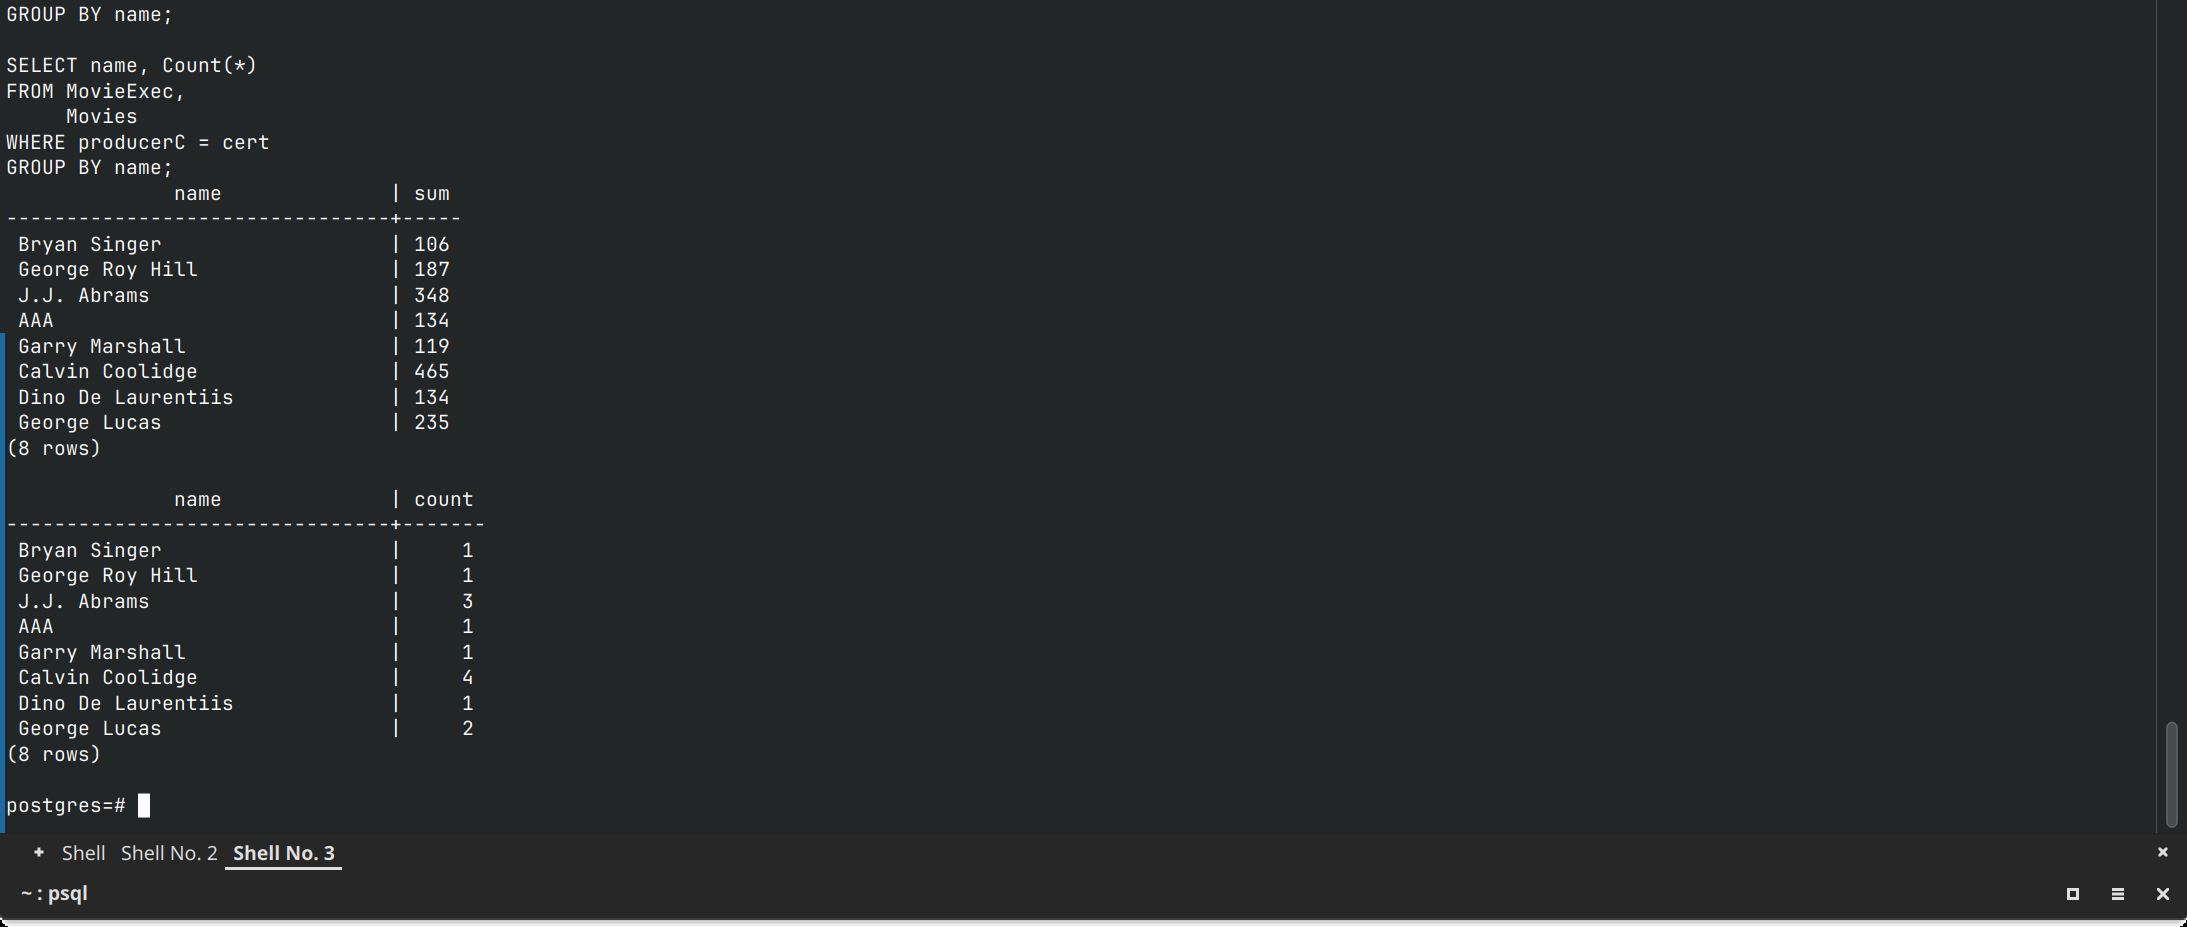
\includegraphics[width=0.8\textwidth]{hw6-4.png}
    \caption{Grouping with More Than One Relation}
    \label{fig:grouping-more}
\end{figure}

\subsection{Having Clause}

\begin{lstlisting}[language=sql]
SELECT name, SUM(length)
FROM MovieExec,
     Movies
WHERE producerC = cert
GROUP BY name
HAVING MIN(year) < 1990;

SELECT name, SUM(length)
FROM MovieExec,
     Movies
WHERE producerC = cert
GROUP BY name
HAVING name like '%o%';
\end{lstlisting}

The execution results are shown in Figure \ref{fig:having-clause}.
\begin{figure}[H]
    \centering
    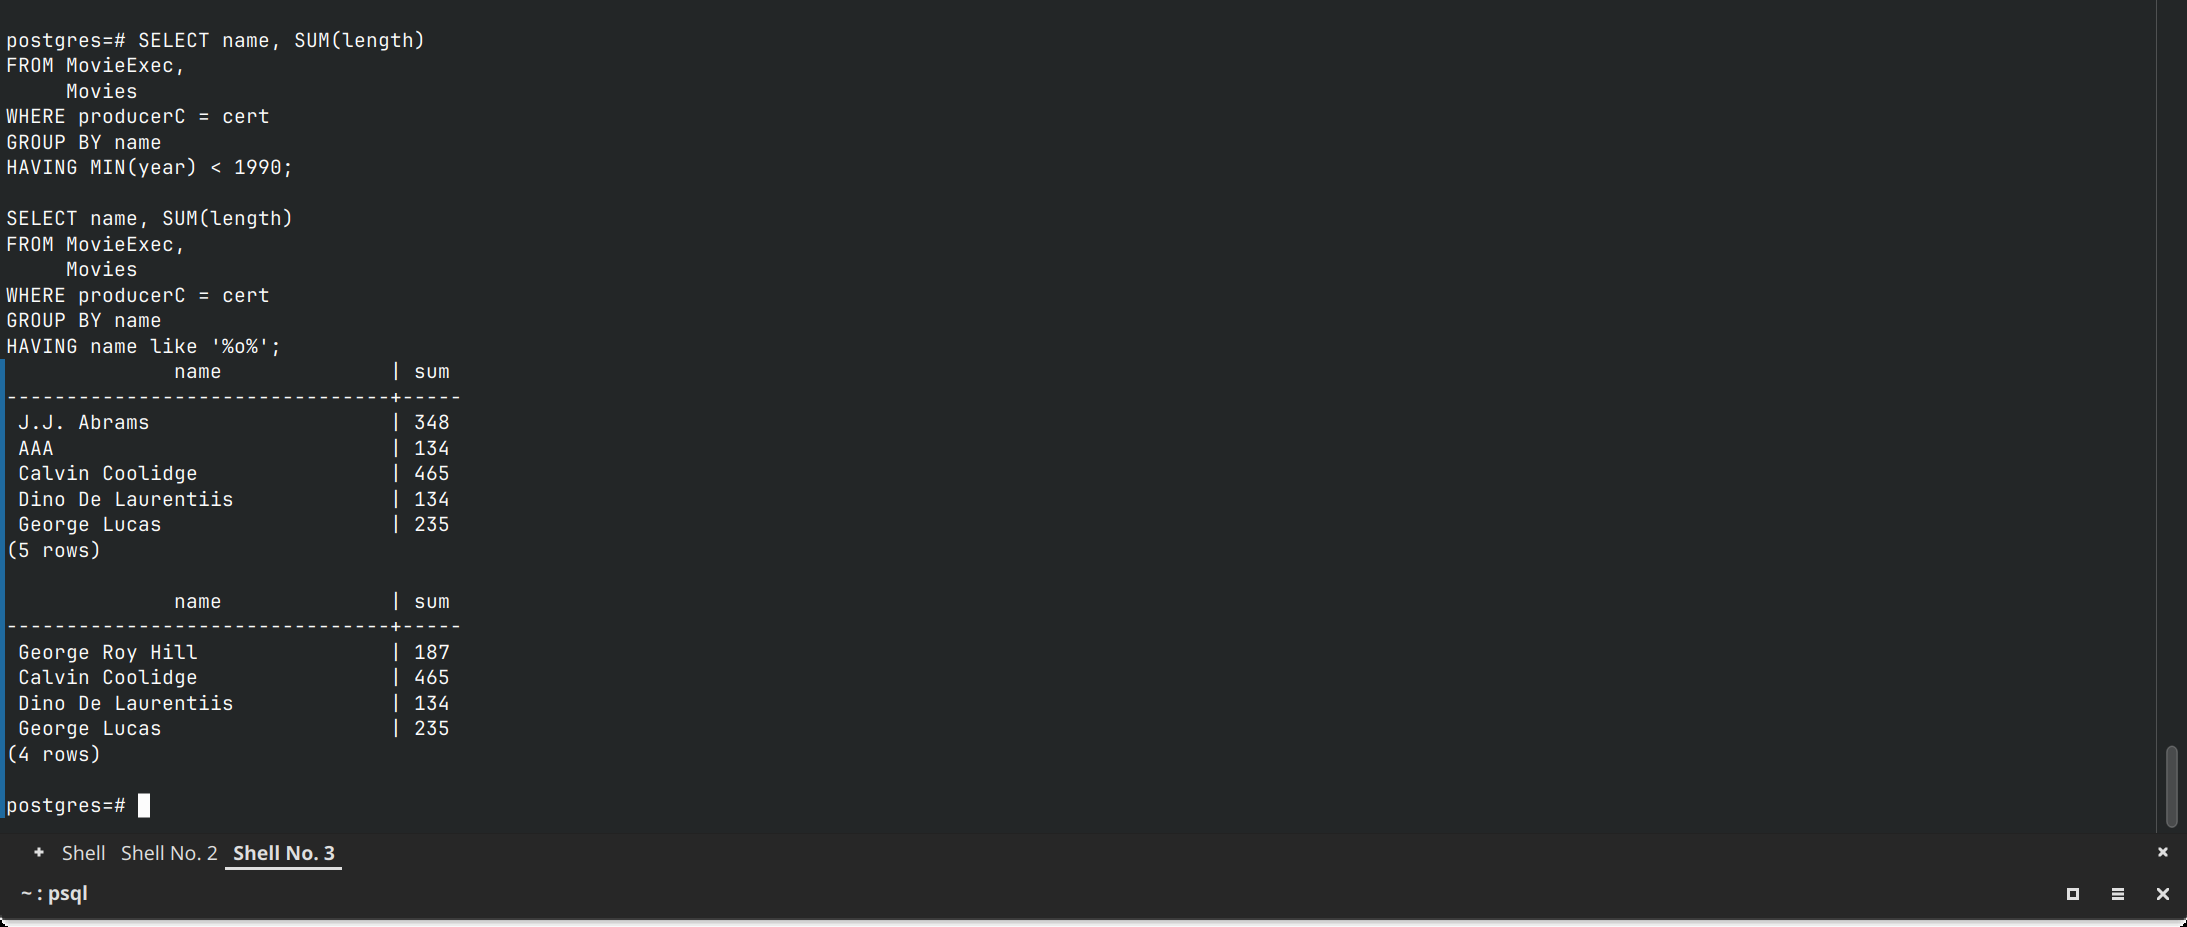
\includegraphics[width=0.8\textwidth]{hw6-5.png}
    \caption{Having Clause}
    \label{fig:having-clause}
\end{figure}

\subsection{Insertion with Subqueries}

\begin{lstlisting}[language=sql]
INSERT INTO Studio(name)
SELECT DISTINCT studioName
FROM Movies
WHERE studioName NOT IN
      (SELECT name
       FROM Studio);
\end{lstlisting}

The execution results are shown in Figure \ref{fig:insertion-subqueries}.
\begin{figure}[H]
    \centering
    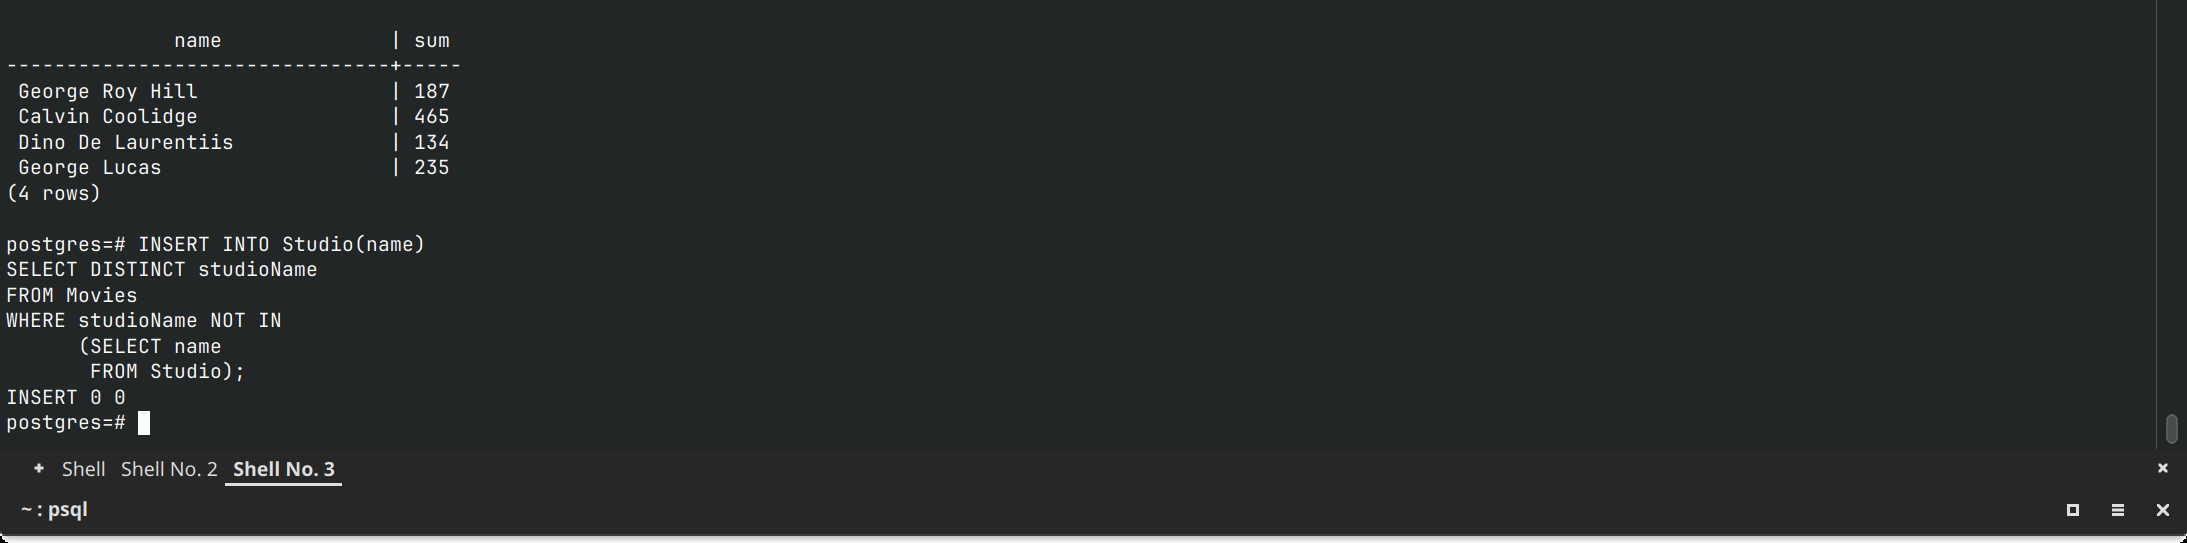
\includegraphics[width=0.8\textwidth]{hw6-6.png}
    \caption{Insertion with Subqueries}
    \label{fig:insertion-subqueries}
\end{figure}

\subsection{Deletion}

\begin{lstlisting}[language=sql]
DELETE
FROM StarsIn
WHERE movieTitle = 'The Maltese Falcon'
  AND movieYear = 1942
  AND starName = 'Sydney Greenstreet';
\end{lstlisting}

the execution results are shown in Figure \ref{fig:deletion}.
\begin{figure}[H]
    \centering
    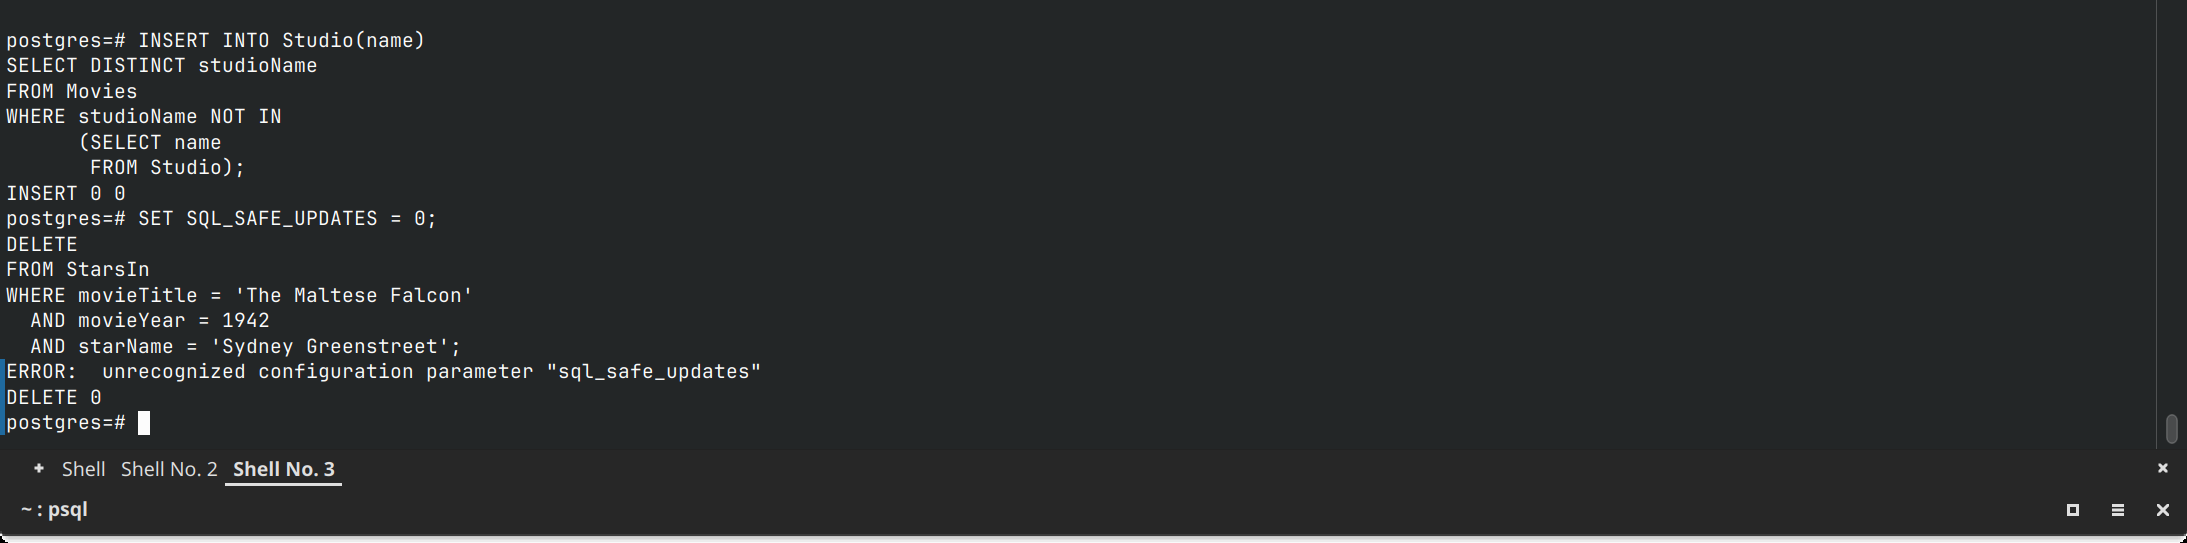
\includegraphics[width=0.8\textwidth]{hw6-7.png}
    \caption{Deletion}
    \label{fig:deletion}
\end{figure}

\subsection{Update}

\begin{lstlisting}[language=sql]
UPDATE MovieExec
SET name = CONCAT('Pres. ', name)
WHERE cert IN (SELECT presC FROM Studio);
\end{lstlisting}

the execution results are shown in Figure \ref{fig:update}.
\begin{figure}[H]
    \centering
    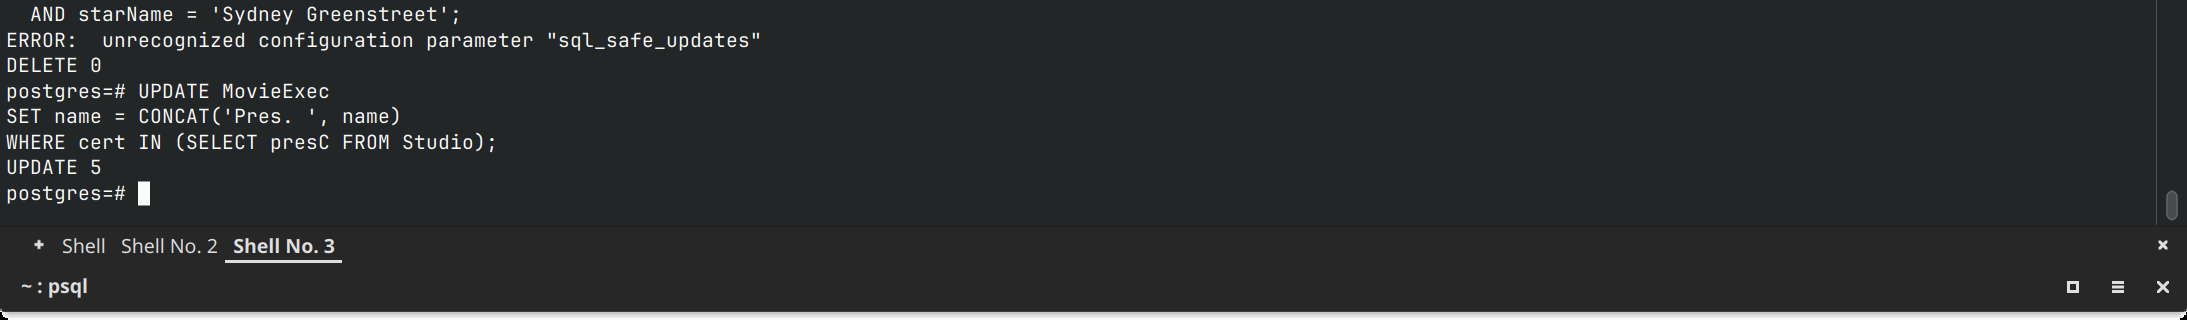
\includegraphics[width=0.8\textwidth]{hw6-8.png}
    \caption{Update}
    \label{fig:update}
\end{figure}

\section{Excerise 6.4.1}
\begin{quote}
    Write each of the queries in Exercise 2.4.1 in SQL, making
    sure that duplicates are eliminated.
\end{quote}
\begin{itemize}
    \item \texttt{Product(maker, model, type)}
    \item \texttt{PC(model, speed, ram, hd, price)}
    \item \texttt{Laptop(model, speed, ram, hd, screen, price)}
    \item \texttt{Printer(model, color, type, price)}
\end{itemize}

\begin{enumerate}
    \item[(a)] What PC models have a speed of at least 3.00?
    \item[(b)] Which manufacturers make laptops with a hard disk of at least 100GB?
    \item[(c)] Find the model number and price of all products (of any type) made by
          manufacturer B.
    \item[(d)] Find the model numbers of all color laser printers.
    \item[(e)] Find those manufacturers that sell Laptops, but not PC's.
    \item[(f)] Find those hard-disk sizes that occur in two or more PC's.
\end{enumerate}

\subsection{Solutions}

\begin{lstlisting}[language=sql]
-- (a) 
SELECT model
FROM PC
WHERE speed >= 3.00;

-- (b)
SELECT DISTINCT maker
FROM Product
JOIN Laptop ON Product.model = Laptop.model
WHERE hd >= 100;

-- (c)
SELECT model, price
FROM Product
WHERE maker = 'B';

-- (d)
SELECT model
FROM Printer
WHERE color = true AND type = 'laser';

-- (e)
SELECT DISTINCT maker
FROM Product
WHERE type = 'laptop'
    AND maker NOT IN (SELECT maker FROM Product WHERE type = 'pc');

-- (f)
SELECT hd
FROM PC
GROUP BY hd
HAVING COUNT(*) >= 2;
\end{lstlisting}

\section{Excerise 6.4.6(a-i)}

Write the following queries, based on the database schema

The database schema is:
\begin{itemize}
    \item \texttt{Product(maker, model, type)}
    \item \texttt{PC(model, speed, ram, hd, price)}
    \item \texttt{Laptop(model, speed, ram, hd, screen, price)}
    \item \texttt{Printer(model, color, type, price)}
\end{itemize}
of Exercise 2.4.1, and evaluate your queries using the data of that exercise.

\begin{enumerate}
    \item[(a)] Find the average speed of PC's.
    \item[(b)] Find the average speed of laptops costing over \$1000.
    \item[(c)] Find the average price of PC's made by manufacturer "A."
    \item[(d)] Find the average price of PC's and laptops made by manufacturer "D."
    \item[(e)] Find, for each different speed, the average price of a PC.
    \item[(f)] Find for each manufacturer, the average screen size of its laptops.
    \item[(g)] Find the manufacturers that make at least three different models of PC.
    \item[(h)] Find for each manufacturer who sells PC's the maximum price of a PC.
    \item[(i)] Find, for each speed of PC above 2.0, the average price.
\end{enumerate}

\subsection{Solutions}

\begin{lstlisting}[language=sql]
-- (a)
SELECT AVG(speed) FROM PC;

-- (b)
SELECT AVG(speed) FROM Laptop WHERE price > 1000;

-- (c)
SELECT AVG(price) FROM PC WHERE model IN (SELECT model FROM Product WHERE maker = 'A');

-- (d)
SELECT AVG(price) FROM (
    SELECT price FROM PC WHERE model IN (SELECT model FROM Product WHERE maker = 'D')
    UNION ALL
    SELECT price FROM Laptop WHERE model IN (SELECT model FROM Product WHERE maker = 'D')
) AS Prices;

-- (e)
SELECT speed, AVG(price) FROM PC GROUP BY speed;

-- (f)
SELECT maker, AVG(screen) FROM Product JOIN Laptop ON Product.model = Laptop.model GROUP BY maker;

-- (g)
SELECT maker FROM Product WHERE type = 'pc' GROUP BY maker HAVING COUNT(DISTINCT model) >= 3;

-- (h)
SELECT maker, MAX(price) FROM Product JOIN PC ON Product.model = PC.model GROUP BY maker;

-- (i)
SELECT speed, AVG(price) FROM PC WHERE speed > 2.0 GROUP BY speed;
\end{lstlisting}

\section{Excerise 6.3.9}
Using the two relations

\begin{itemize}
    \item \texttt{Classes(class, type, country, numGuns, bore, displacement)}
    \item \texttt{Ships(name, class, launched)}
\end{itemize}
from our database schema of Exercise 2.4.3, write a SQL query that will produce
all available information about ships, including that information available in the
C:Casses relation. You need not produce information about classes if there are
no ships of that class mentioned in Ships.

\subsection{Solutions}

\begin{lstlisting}[language=sql]
SELECT 
    Ships.name, 
    Ships.class, 
    Ships.launched, 
    Classes.type, 
    Classes.country, 
    Classes.numGuns, 
    Classes.bore, 
    Classes.displacement
FROM Ships
LEFT JOIN Classes ON Ships.class = Classes.class;
\end{lstlisting}


\end{document}